
\section{Real time scheduling}\label{s:realtime}

There is a way to configure tasks so that Linux enforces global priorities:
processes that run in real time have strict priority over other processes.

Linux implements real time scheduling alongside the usual weighted fair share by
supporting different \textit{scheduling classes}. There are three scheduling
classes that are accessible to users, listed in descending order of priority:
Deadline, Fifo, and Normal. Generally speaking most load is expected to fall
into the Normal scheduling class (hence the name). It is the default scheduling
class, and it is only within the Normal scheduling class that the cgroup
cpu.weight interface is relevant.

Each scheduling class exists completely separately: classes maintain their own
run queues and per-entity state; implement their own scheduling algorithms to
choose from the entities on their runqueue; and balance the load across
runqueues on different cores.

Linux isolates strictly between different scheduling classes: it only schedules
a lower scheduling class if the higher scheduling classes found nothing to run,
and each scheduling class tries to steal work from other cores before returning
that it has nothing to run. It is thereby true that if something in the Normal
scheduling class is running, it means there are no Fifo tasks waiting to run
anywhere on the machine.

This global enforcement is not succeptible to the 4ms granularity. This is
because Linux is also able to schedule at other points in time, not just the 4ms
hardware ticks. These occur when the control flow is in the kernel anyway, and
include the \textit{exit} path, when the running thread blocks, and
\textit{entry}, when a sleeping thread is woken up (via a separate signal, for
example receiving a packet on a listening socket). In these contexts Linux is
able to make fast scheduling decisions, and scheduling at these events is
sufficient to enforce isolation: the tick-based preemption granularity is
relevant for latencies of the processes within a priority, but isolating across
priorities only requires the correct scheduling decision to be made on entry and
exit. 

\begin{figure}[t]
    \centering
    \begin{subfigure}[t]{0.48\columnwidth}
        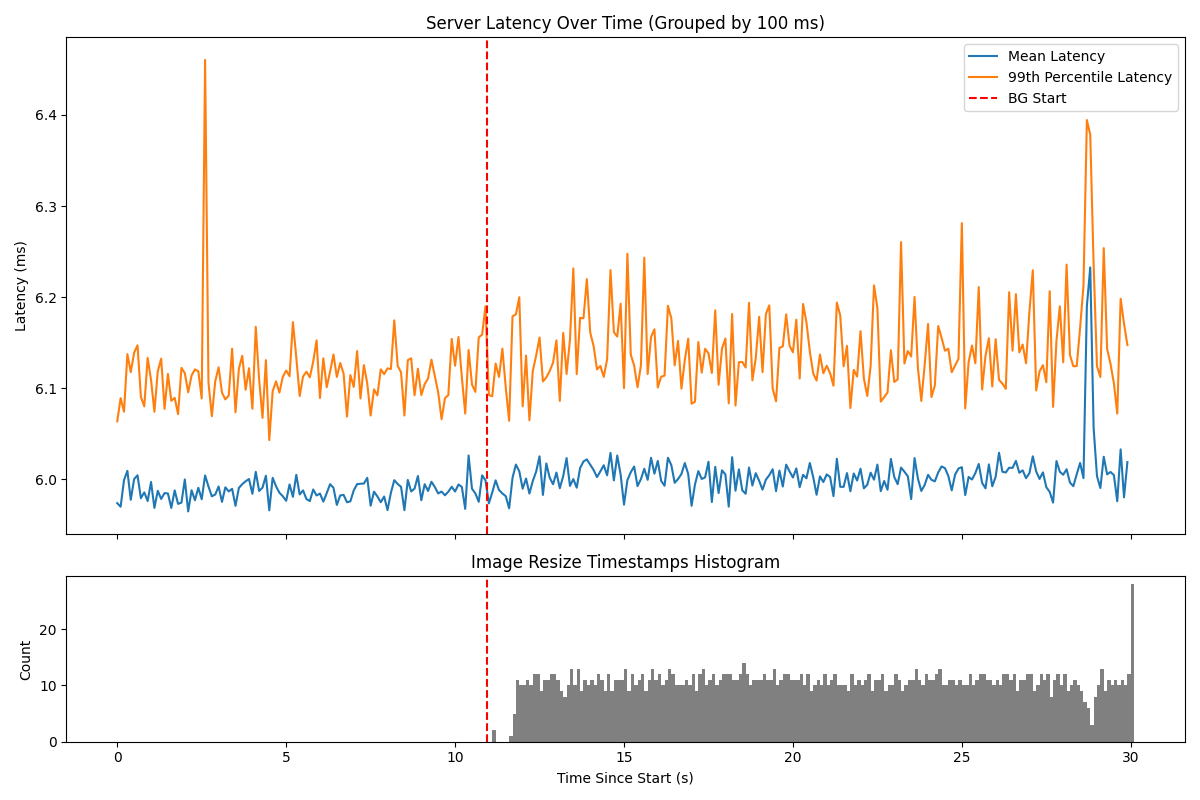
\includegraphics[width=\columnwidth]{graphs/unedited-rt-low-two.png}
        \caption{Low load}\label{fig:unedited-rt-low-two}
    \end{subfigure}
    \hspace{\fill}
    \begin{subfigure}[t]{0.48\columnwidth}
        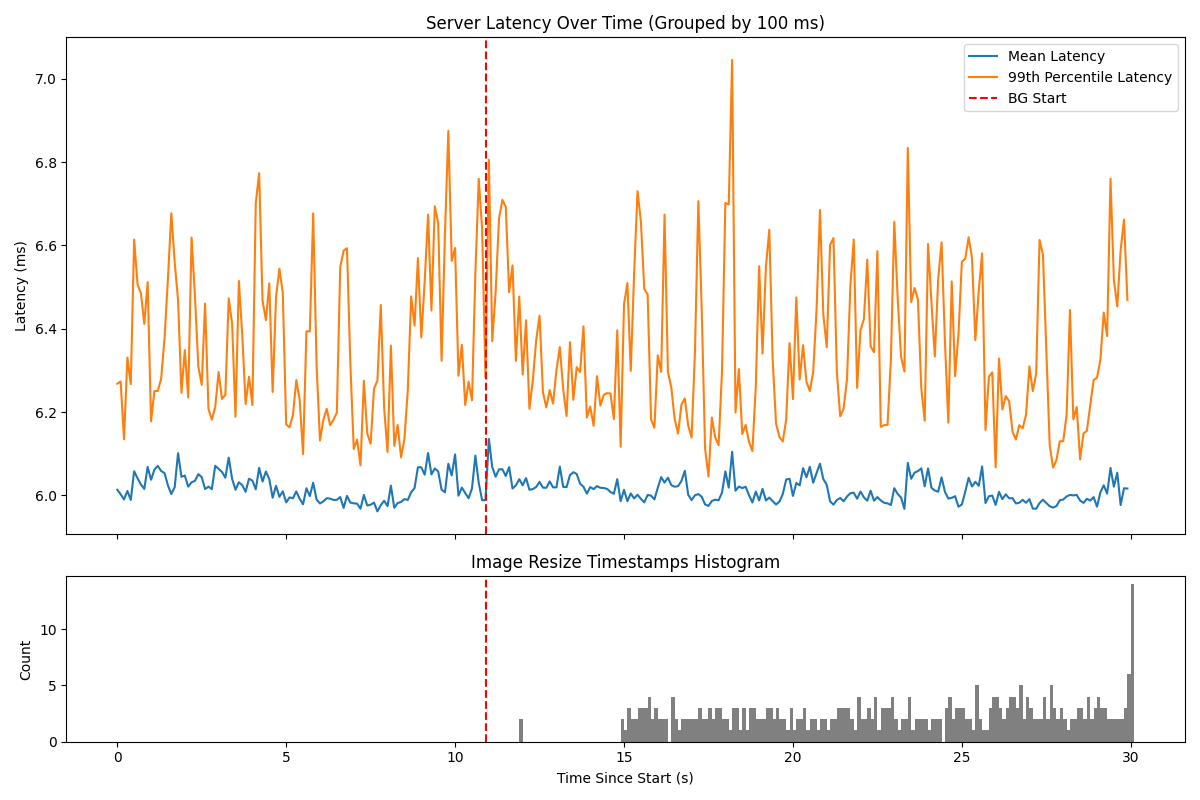
\includegraphics[width=\columnwidth]{graphs/unedited-rt-high-two.png}
        \caption{High load}\label{fig:unedited-rt-high-two}
    \end{subfigure}
    \vspace{4pt}
    \caption{Results of the same experiment, with LC running as a real time process}\label{fig:unedited-rt}
\end{figure}

This points to a possible solution: run LC in a realtime scheduling class and BE
in Normal. The Deadline class requires processes to specify a runtime $r$,
deadline $d$, and a period $p$; it guarantees that each process will get $r$
cputime by $d$, every $p$ time. So if the $r$ is 2ms, $d$ is 3, and $p$ is 10,
the Deadline scheduler guarantees that the process will get 2 ms every 10ms,
within 3ms of the period starting. The Deadline scheduler does admission control
in order to be able to make these guarantees. The Fifo scheduling class, on the
other hand, allows for oversubscription. It is a priority scheduler: it has 99
priorities, each takes strict precedent over the one lower; within priorities
the scheduler enforces a global first-in-first-out (hence the Fifo class name),
based on when processes become runnable.

So, we run the same experiment as in \autoref{s:intro}, but put the
LC task in the Fifo scheduling class, and don't put the BE tasks into groups.
Doing so effectively promotes the latency criticality of the LC task in the eyes
of the system, and makes use of Linux's strong isolation of real time workloads.
\autoref{fig:unedited-rt} shows the resulting measured latencies in the same
low and high load setting as previously. We see much stabler latencies, as
expected; in the baseline as well as once the BE tasks are started. This looks
promising on two fronts: 1: we get better isolation by making use of Linux's
strict boundaries between scheduling classes, and 2: we see improved tail
latency for the LC task because of the fifo run-to-completion scheduling
algorithm.

\begin{figure}[t]
    \centering
    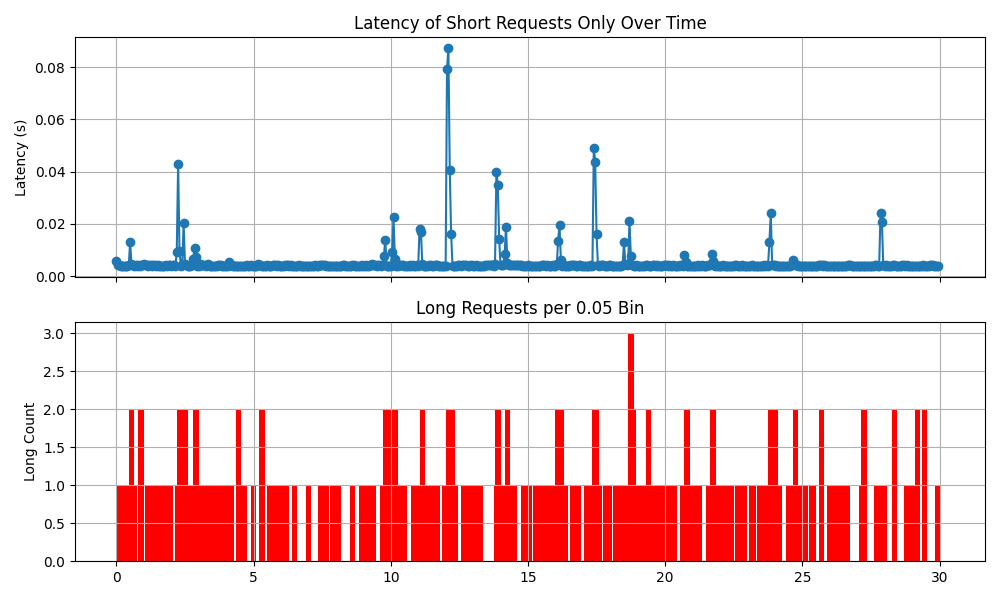
\includegraphics[width=\columnwidth]{graphs/hol-blocking.png}
    \caption{Blah blah blah}\label{fig:hol-blocking}
\end{figure}


However, the observed improved tail latency is actually a side-effect of the
experimental setup, where each request does the exact same thing and processing
times are uniform. Fifo's run-to-completion scheduling is known to have a
failure mode of head-of-line (HoL) blocking, where long-running requests
monopolize the CPU while short requests wait in the queue. This leads to much
worse tail latencies for short requests, at the expense of long requests being
slightly faster (proprtionally a smaller amount than the short requests are
waiting). We can see this phenomenon in a separate experiment, where we make a
small percentage (2\%) of requests take longer, and then graph the latencies of
only the short requests. Figure~\ref{fig:hol-blocking} shows the results, we can
see exactly when there are enough long requests that all the cores are blocked
processing them and the short requests' latencies spike. In real applications
requests almost always have a distribution of runtimes, sometimes long-tailed
sometimes short-tailed, but definitely enough of a tail that head-of-line
blocking would become a problem.

Solving the problem of HoL blocking is possible but requires knowing about
expected processing times and ensuring that requests on the same core have about
the same processing time. There is related work that does this~\cite{TODO}; but
requires a whole distributed infrastructure. The solution approach of using the
Fifo scheduler would thus require a whole infrastructure above it to minimize
the variance of processing times on cores/machines; given the original problem
was separating the LC and BE worklaods on a machine, this moves beyond the scope
of the problem.

The solution is also overkill in another dimension: Fifo enforces not only
cross-core isolation between different priorities, but also within the same
priority. This means that Linux is performing balancing and potentially
migration almost every time an LC thread wakes up or exits; in order to ensure
that the next process the core runs is next in the global fifo ordering. This
requires the scheduling core to potentially lock the runqueues of all the other
cores as it ensures the task it will run the next is the one with the highest
priority, and within that priority the once that first became runnable.\hmng{the
uptick was visible in the last graph, I think because of the spikes now it's
not. Should I try stuff to see if I can get that back?}

We conclude that the Fifo scheduling class is not a good solution: although it
is able to globally ensure isolation between LC and BE tasks, its scheduling
time overheads and algorithm make in poorly suited for a production setting.



